\documentclass[10pt]{article}

\usepackage[document]{ragged2e}

% for pdflatex
\usepackage[utf8]{inputenc}
% for hyperlink
\usepackage{hyperref}
\hypersetup{
    colorlinks=true,
    linkcolor=blue,
    filecolor=magenta,
    urlcolor=cyan,
}
% for table spanning multiples pages
\usepackage{longtable}
% for custom enum
\usepackage{enumitem}
% for removing alinea begin of paragraph
\usepackage{parskip}
\usepackage{array, xcolor, graphicx}
\usepackage[a4paper, margin=1cm]{geometry}
\title{\bfseries{\huge{Blockchain \& Data Science Engineer}}\\[0.75cm] \Large{4 years of experience in blockchain and cryptocurrencies} }
% no author
\author{\bfseries\Huge \vspace{-4ex}}
% no date
\date{}
% custom for column style
\definecolor{lightgray}{gray}{0.8}
% custom for column type
\newcolumntype{L}{p{0.2\textwidth}}
% custom for column type
\newcolumntype{R}{p{0.75\textwidth}}
% custom for column type
\newcommand\VRule{\color{lightgray}\vrule width 2pt}
% for bullet point outside of list
\newcommand{\tabitem}{~~\llap{$\rightarrow$}~~}
\begin{document}

\begin{minipage}[t]{0.80\textwidth}
\textbf{\Large{Mohamed Amine LEGHERABA}}\\
\vspace{4ex}26 years old\\
92 bis rue Rouget de Lisle, Bezons, France\\
\href{tel:+33630829000}{+33 6 30 82 90 00}\\
\href{mailto:mlegheraba@protonmail.com}{mlegheraba@protonmail.com}\\
\href{https://github.com/MohamedLEGH}{github.com/MohamedLEGH}\\
\vspace{5ex}{\bf French}: native\\
{\bf Anglais}: fluent (TOIEC: 935)\\
\end{minipage}
\begin{minipage}[t]{0.20\textwidth}
\vspace{-3ex}
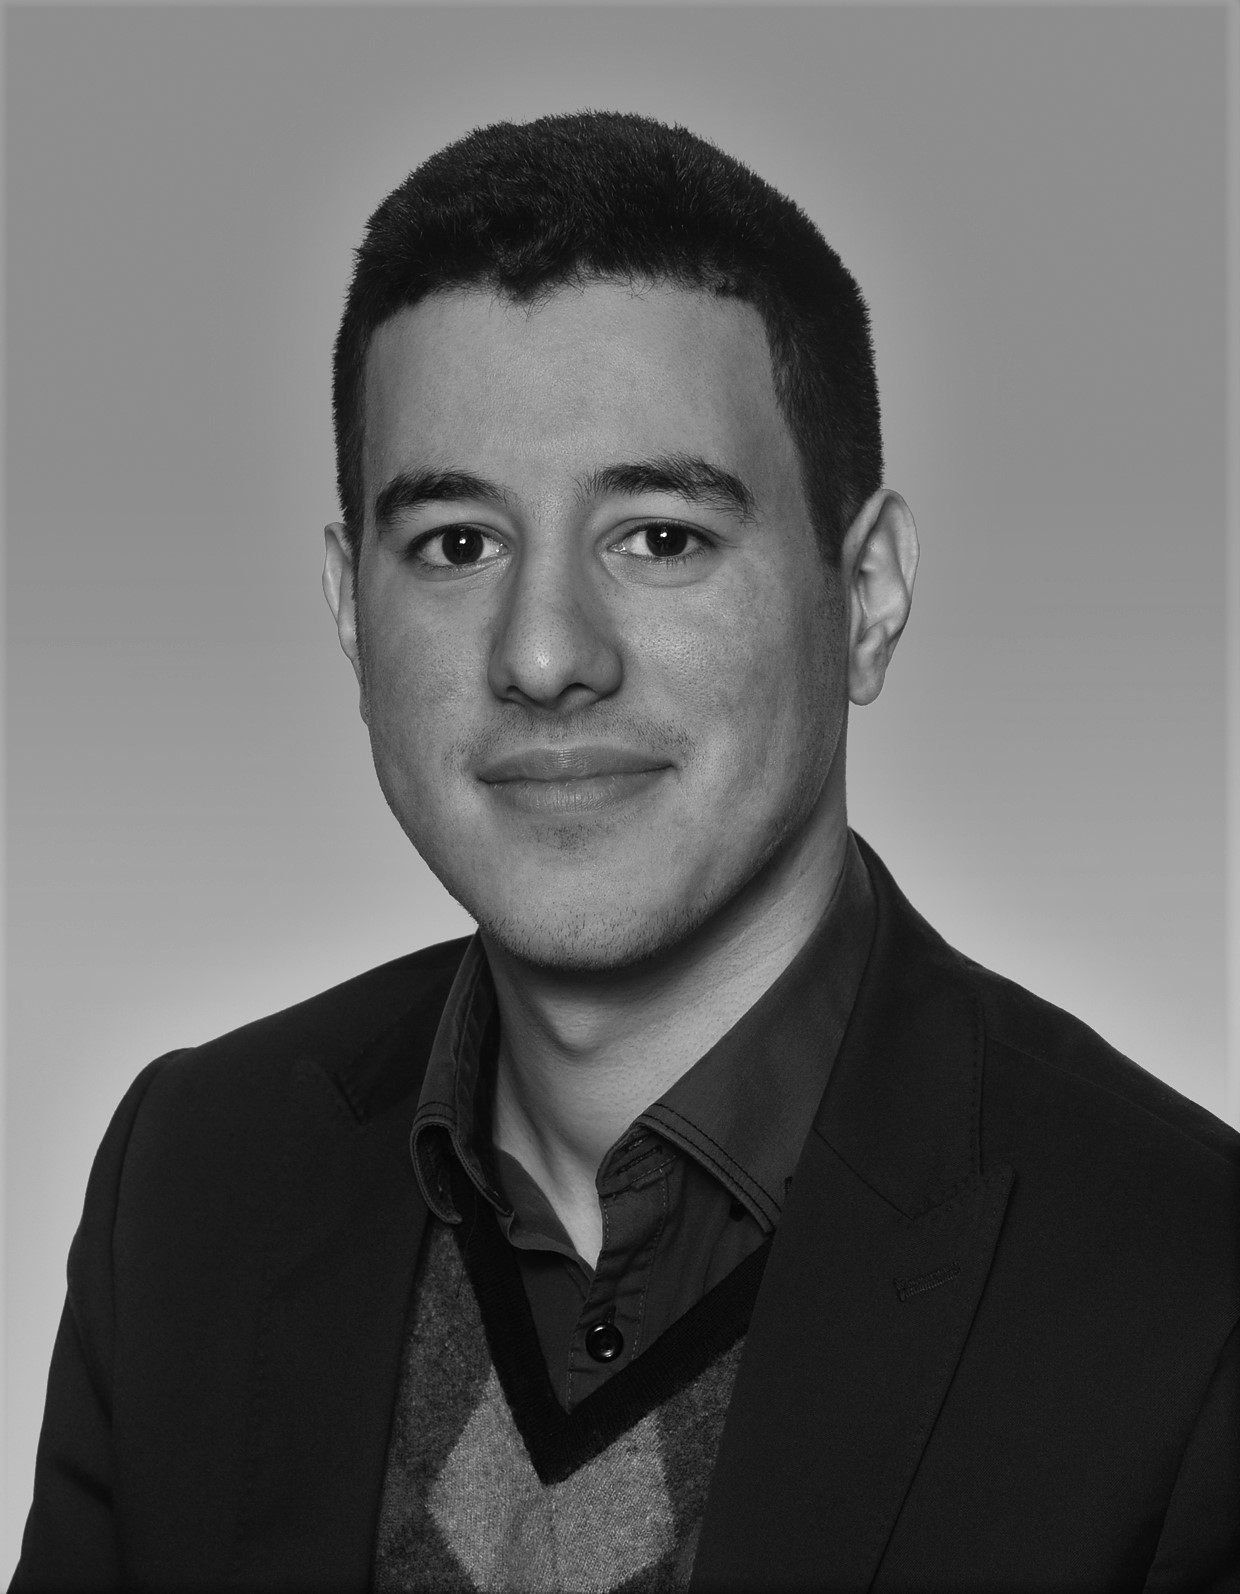
\includegraphics[width=4cm]{figures/Legheraba-Mohamed-White.jpg}
\end{minipage}
% to make maketitle work without begin of page
{\let\newpage\relax\maketitle}
% to remove page number
\thispagestyle{empty}

\vspace{-10ex}

\section*{Formation}

\vspace{2ex}

\begin{tabular}{L!{\VRule}R}
\textbf{\textit{2015--2018}} \hspace{1.5ex} 
\includegraphics[width=1.4cm]{figures/Logo_Reseau_Polytech.png} & \textbf{Engineering degree, Polytech Sorbonne}, speciality \textit{Applied mathematics and computer science}: Statistics, Differential equations, Programmation, Data structures, Parallelism.\\[0.75cm]
\textbf{\textit{2017 (Winter)}} \hspace{.5ex} 
\includegraphics[width=.85cm]{figures/TU.png} & \textbf{Erasmus semester at TU Delft}, Netherlands: Graph theory, Cryptography, Blockchain, Cloud Computing, Data Visualization.\\[0.75cm]
\textbf{\textit{2013--2015}} \hspace{5ex} 
\includegraphics[width=.85cm]{figures/PEIP_logo.png}  & \textbf{Polytech Sorbonne},  \textit{PeiP} (Parcours des écoles d'ingénieurs Polytech): Maths, Computer Science, Physics, Chemistry, Mechanics.\\[0.75cm]
\textbf{\textit{2013}} & \textbf{Baccalaureate}, in Science, passed with honours, Lycée Chaptal. \\
\end{tabular}

\vspace{2ex}

\section*{Work Experience}

\vspace{2ex}

\begin{longtable}{L!{\VRule}R}
\textbf{\textit{Since April 2019}}& 
\includegraphics[width=2cm]{figures/SIA_logo.png} \hspace{0.2cm} {\bf Blockchain \& Data Science Engineer, Sia Partners, ongoing.} \\[0.25cm]

& \tabitem \small{\textbf{CBDC experimentations at Banque de France} (member of the blockchain unit as a blockchain technical expert, technical lead for 1 experimentation, technical support for 2 other experimentations, training for other team members about Blockchain and DevOps, implementation of the CI/CD pipelines)}

\\[0.20cm]
& \tabitem \small{\textbf{Monitoring of trading limits using a blockchain network for an investment fund} (blockchain expert, implementation of a private blockchain network, development of smart contracts and of an oracle, code review, supervision, testing) \it{Mission found and won by myself thanks to my network}}

\\[0.20cm]
& \tabitem \small{\textbf{Creation of a payment mobile application in cryptocurrencies for a French retailer} (blockchain expert, development of a secure payment interface in cryptocurrencies, development of a back office application and a cold wallet for the secure management of cryptocurrencies and their exchange for euros)}

\\[0.20cm]
& \tabitem \small{\textbf{Recording of patient consent on the blockchain with digital signatures for a public sector actor} (in the context of clinical trials, implementation of an interface to collect the digital signatures of the patient and the doctor, sending of the hash of the signatures on the Ethereum network, web interface to check the validity of the registration)}

\\[0.20cm]
& \tabitem \small{\textbf{Certification of the decibel level on the Ethereum network for a transportation operator} (IoT \& Blockchain, reception of decibel data with a Bluetooth socket, transfer of the information on the blockchain when the value exceeds the limit, display of values in real time on the web interface)}

\\[0.20cm]
& \tabitem \small{\textbf{Smart Data Quality: Software to clean and visualize data to help the consultant during his mission} (development of data science algorithms in Python, optimization of code, deployment on AWS infrastructure, ...)}

\\[0.20cm]
& \tabitem \small{\textbf{Heka Project: \href{https://heka.sia-partners.com/en}{Software factory} for Data Science applications} (development of microservices in Python and React, continuous deployment on the Kubernetes infrastructure, ...)}

\\[0.20cm]
& \tabitem \small{\textbf{R\&D watch on blockchain, cryptocurrencies and distributed systems} (study of Liquid, Libra and TON blockchain networks, Lightning Network, HTLC Atomic Swap, Zero-knowledge proofs, Raft protocol, Taproot and Multi-Party Computation technologies, ...)}

\\[0.20cm]
& \tabitem \small{\textbf{Writing articles} (\href{https://www.sia-partners.com/fr/actualites-et-publications/de-nos-experts/la-blockchain-catalyseur-de-la-decentralisation-et-de-la}{\textit{Blockchain \& 5G}}, \href{https://www.sia-partners.com/fr/actualites-et-publications/de-nos-experts/entretien-avec-pierre-noizat-bitcoin-et-cryptomonnaies-0}{\textit{Interview with Pierre Noizat}}, ...)}

\\[0.20cm]
& \tabitem \small{\textbf{Course \textit{Programming a blockchain}} (\href{https://github.com/MohamedLEGH/tutoriel-blockchain-creation-bootstrap}{Polytech Sorbonne}, \href{https://github.com/MohamedLEGH/tutoriel-blockchain-MinesBootstrap}{Mines St Etienne}, ...)}

\\[0.20cm]
\textbf{\textit{March--September 2018}}& 
\includegraphics[width=1.5cm]{figures/ofi-am.png} \hspace{0.2cm} {\bf Blockchain \& Cloud R\&D watch intern, Development Department, OFI AM, 6 months}.\\
& \small{Watch around Blockchain technologies, task automation with Airflow, application containerisation with Docker and system supervision with Tableau Server.} \\

\\[0.20cm]
\textbf{\textit{2017}}& {\bf Development during multiples ICO, of which 2 have raised more than \$5M}.\\
& \small{Development of smart contracts for the token of the ICOs, building of a security protocol to store the tokens, creation of scripts to interact with the Ethereum network.} \\


\end{longtable}

\vspace{2ex}

\section*{Technical Skills}

\vspace{2ex}

\begin{tabular}{ l l }
\textbf{Blockchain}: Ethereum, Corda, Hyperledger, Bitcoin & \textbf{DevOps}: Kubernetes, Gitlab CI/CD, GCP, Terraform \\[0.1cm]
\textbf{Smart contracts}: Solidity, Corda contrats, Chaincodes & \textbf{Tools}: Shell, Git, Docker, VS Code, PowerPoint \\[0.1cm]
\textbf{Mathematics}: Cryptography, Statistics, Graphs & \textbf{Programming}: Python, JavaScript, Bash, C/C++, Kotlin, R \\[0.1cm]
\textbf{Databases}: PostgreSQL, MySQL, SQLAlchemy & \textbf{Frameworks}: ReactJS, Node.js, Ethers.js, Flask, Web3.py, PyQt \\[0.1cm]
\textbf{Protocols}: Lightning Network, IPFS, TCP/IP & \textbf{Methodology}: Agile Method, APIs REST, Microservices \\[0.1cm]
\end{tabular}

\vspace{2ex}

\section*{Functional and Business Skills}

\vspace{2ex}

\begin{tabular}{ l }
\textbf{Publics \& Private blockchain networks}: When to use a public versus a private network, differences between frameworks.\\[0.1cm]
\textbf{Decentralized finance} : Stablecoins, Defi protocols, securing private keys, connexion with traditional finance.\\[0.1cm]
\textbf{CBDC \& Financial Market Infrastructures}: Implications of a crypto euro, Target2 \& Target2 Securities, PvP \& DvP.\\[0.1cm]
\textbf{Audit}: Audits of smart contracts, audits of blockchain technologies, audits of Blockchain startups \& fintechs.\\[0.1cm]
\end{tabular}

\vspace{1ex}

\section*{Volunteer Experience}

\vspace{2ex}

\begin{tabular}{L!{\VRule}R}
\textbf{\textit{Since 2018}} & Association \textbf{Le Trait D’Union}, Homework help for high school and college students. Writing grant applications, treasurer. \\[0.75cm]

\textbf{\textit{2014--2017}} & Student association \textbf{Averroès}, Food donations for students, treasurer then president. \\
\end{tabular}

\vspace{2ex}

\section*{Interests}

\vspace{2ex}

\hspace*{1ex} \textbf{Electronics} (retrogaming console with a Raspberry Pi, fan control using a transistor, ...) \\
\hspace*{1ex} \textbf{Study of socio-economic doctrines} (liberalism, Austrian school of economics, anarchism, technoethics, ...) \\
\end{document}
